% 1958 年广东卷第 3 题：⊙O 中弦 AB、AC，D 为弧 AB 中点、E 为弧 AC 中点，DE 交 AB 于 M、交 AC 于 N（按源卷布局）
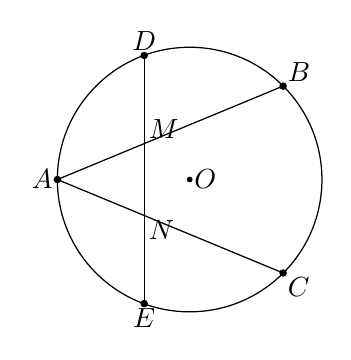
\begin{tikzpicture}[scale=1.05, line width=0.45pt,
  every node/.style={inner sep=1.5pt}]
  \coordinate (O) at (0,0);
  \coordinate (A) at (-1.6,0);
  \coordinate (D) at (-0.55,1.5);
  \coordinate (E) at (-0.55,-1.5);
  \coordinate (B) at (1.13,1.13);
  \coordinate (C) at (1.13,-1.13);
  \coordinate (M) at (-0.55,0.44);
  \coordinate (N) at (-0.55,-0.44);
  \draw (O) circle (1.6);
  \draw (D) -- (E);
  \draw (A) -- (B);
  \draw (A) -- (C);
  \fill (A) circle (1.3pt);
  \fill (B) circle (1.3pt);
  \fill (C) circle (1.3pt);
  \fill (D) circle (1.3pt);
  \fill (E) circle (1.3pt);
  \fill (O) circle (1pt);
  \node[anchor=east] at (A) {$A$};
  \node[anchor=south] at (D) {$D$};
  \node[anchor=north] at (E) {$E$};
  \node[anchor=south west] at (B) {$B$};
  \node[anchor=north west] at (C) {$C$};
  \node[anchor=south west] at (M) {$M$};
  \node[anchor=north west] at (N) {$N$};
  \node[anchor=west] at (O) {$O$};
\end{tikzpicture}
